%------------------------------------------
%
%Paper to be submitted to: 
%Paper title: Development of the Open-Source Fuel Cell Simulation Toolbox (OpenFCST) Framework
%Paper Number: 
%Version 
%
%------------------------------------------

\documentclass[]{elsart}


% Include packages
\usepackage[]{cite}
\usepackage[]{amsmath} %for math
\usepackage[]{graphicx} %for graphics
\usepackage{nomencl} %for nomenclature
\usepackage{setspace} %for double spacing

% Define commands to assure consistent treatment throughout document
%\newcommand{\eqnref}[1]{(\ref{#1})}
%\newcommand{\class}[1]{\texttt{#1}}
%\newcommand{\package}[1]{\texttt{#1}}
%\newcommand{\file}[1]{\texttt{#1}}
%\newcommand{\BibTeX}{\textsc{Bib}\TeX}
\renewcommand{\vec}[1]{\mathbf{#1}}
\providecommand{\abs}[1]{\lvert#1\rvert}
\providecommand{\norm}[1]{\lVert#1\rVert}
\renewcommand{\thefootnote}{\fnsymbol{footnote}}

\RequirePackage{ifthen}
\renewcommand{\nomgroup}[1]{%
\ifthenelse{\equal{#1}{G}}{\item[\textbf{Greek Letters}]}{%
\ifthenelse{\equal{#1}{A}}{\item[\textbf{}]}{}}}

% Journal where the paper is submitted:
\journal{Journal of Power Sources}

% To create a nomenclature. Once I have run the latex file I have to type in the xterm once inside this directory:
%lisboa:~/Documents/My_Papers/2006/Electrochimica_Acta_Jan06 secanell$ makeindex Secanell_EA_05_Numericao_Optimization_of_a_PEMFC_Cathode_Electrode.nlo -s nomencl.ist -o Secanell_EA_05_Numericao_Optimization_of_a_PEMFC_Cathode_Electrode.nls
%to create the .nls file needed to create the nomenclature
\makenomenclature

%---------------------------------------------
%---------------------------------------------
\begin{document}

%---------------------------------------------
%---------------------------------------------
\begin{frontmatter}

\title{OpenFCST: An open-source fuel cell simulation toolbox for polymer electrolyte fuel cell analysis}

\author[ESDLab]{M. Secanell\corauthref{cor}},
\ead{secanell@ualberta.ca}
\author[ESDLab]{M. Bhaiya},
\author[ESDLab]{V. Zingan},
\author[ESDLab]{P. Wardlaw} and
\author[AFCC]{A. Putz} 

\corauth[cor]{Corresponding author.}
\address[ESDLab]{Energy Systems Design Laboratory, Department of Mechanical Engineering, University of Alberta, Edmonton, AB, Canada}
\address[AFCC]{Automotive Fuel Cell Cooperation Corp., Burnaby, BC, Canada}
 
%---------------------------------------------
%---------------------------------------------
%\begin{frontmatter}

\begin{abstract}

An overview to the open-source Fuel Cell Simulation Toolbox (OpenFCST) is provided. an extendable, general purpose fuel cell simulation software written in C++.

%deal.II overview paper example ( DOI:10.1145/1268776.1268779 OR http://dl.acm.org/citation.cfm?doid=1268776.1268779):

%An overview of the software design and data abstraction decisions chosen for deal.II, a general purpose finite element library written in C++, is given. The library uses advanced object-oriented and data encapsulation techniques to break finite element implementations into smaller blocks that can be arranged to fit users requirements. Through this approach, deal.II supports a large number of different applications covering a wide range of scientific areas, programming methodologies, and application-specific algorithms, without imposing a rigid framework into which they have to fit. A judicious use of programming techniques allows us to avoid the computational costs frequently associated with abstract object-oriented class libraries.

%The paper presents a detailed description of the abstractions chosen for defining geometric information of meshes and the handling of degrees of freedom associated with finite element spaces, as well as of linear algebra, input/output capabilities and of interfaces to other software, such as visualization tools. Finally, some results obtained with applications built atop deal.II are shown to demonstrate the powerful capabilities of this toolbox.



Keywords: fuel cell, catalyst layer, gas diffusion layer, platinum loading, sensitivity analysis, finite elements
\end{abstract}

\begin{keyword}
    fuel cell, catalyst layer, gas diffusion layer, platinum loading, sensitivity analysis, finite elements
\end{keyword}

\end{frontmatter}

%----------------------------------
%----------------------------------
\section{Introduction}  

Reducing production cost and improving performance, reliability and durability remain critical prerequisites for commercialization of polymer electrolyte membrane fuel cells. Past investigations on electrode design for optimal performance \cite{Sasikumar04,Passalacqua01,Antolini99,Xie05,Gode03} and low platinum loading \cite{Cunningham03,Mukerjee93,Madhu06} have been mainly based on trial-and-error and parametric studies. When the number of design variables becomes large, a more systematic and rational approach to optimization of the electrode structure and composition is necessary. One such case is when trying to design a complete membrane electrode assembly (MEA). 
 
 The anode and cathode gas diffusion layer (GDL) and catalyst layer (CL) have multiple functions that require a combination of different materials and structures. For example, in the GDL, the electron conductive material provides the necessary electrical conductivity, while the porous structure allow reactant transport. In order for the fuel cell to provide the best possible performance at a minimum cost, the optimal porosities and amounts of different materials in the GDL and CL need to be determined. Since all these design parameters are coupled, the task of finding the optimal amount of material to reduce production cost and maximize performance becomes in fact a multi-objective, multi-variable problem that depends on the fuel cell operating and geometric conditions. To date, only four research groups - Song et al. \cite{Song04,Song05}, Grujicic et al. \cite{Grujicic04,Grujicic04_2,Grujicic04_3}, Mawardi et al. \cite{Mawardi05} and Secanell et al. \cite{Secanell06,Secanell07a,Secanell07b,Secanell07c} - have attempted to perform single cell fuel cell optimization using a physical or theoretical model. In all cases, a {\em single objective} optimization problem was solved and only Song et al. \cite{Song04,Song05} and Secanell et al. \cite{Secanell06,Secanell07a,Secanell07b,Secanell07c}, have attempted to optimize electrode composition by using a one-dimensional cathode model and a two-dimensional cathode and anode model respectively.

In this paper, a numerical optimization methodology recently developed by the authors \cite{Secanell07a,Secanell07b} and used to investigate the optimal cathode composition of standard fuel cells is extended to allow determination of the optimal composition and structure of an entire membrane electrode assembly. Section \ref{sec:MEA} of this paper describes the MEA model. Section \ref{Optimization} presents the optimization formulation and the computational framework. Using the computational framework, a multi-objective problem is solved and Pareto fronts for cost and performance are obtained in section \ref{sec:applications}, and the amounts of ionomer or electrolyte, platinum and carbon in both the anode and cathode CLs and the porosities in the GDL  determined from the optimization process are presented and analyzed. The results demonstrate the importance of using a multi-objective formulation and highlight in particular the trade-offs between cost and performance. To the knowledge of the authors this represents the first attempt in the literature to apply numerical optimization to solve a multi-objective optimization problem for a complete membrane electrode assembly.

%------------------------------------------
\section{Software overview}


%------------------------------------------
\subsection{Application classes}

%------------------------------------------
\subsection{Equation classes}

%------------------------------------------
\subsection{Layer classes}

OpenFCST contains several classes that 


\subsubsection{Micro-scale integration}



%------------------------------------------
\subsection{Material classes}

%------------------------------------------
\section{Interfaces to Other Software}

\subsection{Pre-processing}
Salome

\subsection{Analysis}

deal.ii
COLDAE

\subsection{Post-processing}
OpenFCST contains a suite of post-processing routines in order to compute post-processing functions at each degree of freedom in the finite element domain and functionals evaluated over a layer. These functions and functionals are critical for analyzing fuel cell operation and can be used as design objectives as described in references \cite{Secanell07a,Secanell07b,Secanell07c}. Functions that can be evaluated at each degree of freedom during post-processing include relative humidity, volumetric current density, agglomerate effectiveness, water sorption and desorption, heating source terms such as joule heating and entropic heating and so on. Functionals that can be evaluated witin the OpenFCST framework include: anode and cathode catalyst layer current density, water adsoption and desorption into the membrane and heat generation in the electrode.

In order to visualize the solution at each degree of freedom over the domain, OpenFCST uses the deal.II output modules in order to output the solution to a variety of formats including: VTK [Schroeder et al. 2004], OpenDX in both text and binary format, UCD format for AVS Express, binary and text files for Tecplot, gnuplot, povray, encapsulated postscript, and GMV. The developers recommend the use of Paraview

\subsection{Design}

Dakota

\subsection{Test Driven Development}



%------------------------------------------
\section{Documentation} \label{sec:Documentation}

OpenFCST is distributed with documentation explaining abstract and working class public and internal interfaces, and a detailing their usage and the interplay between different classes and namespaces.

The documentation is divided in two major components. The first part is a user guide including several tutorials on how to compile and run the applications. 

The second part is a web-based handbook describing all classes and functions of OpenFCST. It is produced directly from the source code using the documentation tool DOxygen \cite{}. It provides a detailed interface for each class in the library as well as inheritance diagrams in order to highlight the connections between different classes of the software. 

%------------------------------------------
\section{Case Studies} \label{sec:Case_studies}

\begin{itemize}
 \item Cathode application
 \item Membrane electrode assembly application
 \item Fluid flow solver (channel)
\end{itemize}


\subsection{Membrane Electrode Assembly Model} \label{sec:CS:MEA}
  In this section, a model accounting for the salient transport phenomena in a complete membrane electrode assembly is outlined. A complete description of the fuel cell model is given in previous work \cite{Secanell07_thesis,Secanell07a,Secanell07b}. The model considers a two-dimensional section of the fuel cell and is based on the following assumptions: 
\begin{itemize}
	\item The fuel cell is at steady state and operates at constant temperature and pressure.
	\item The cathode is fed with humidified air.
	\item The anode is fed with humidified hydrogen.
	\item The gas diffusion layers are composed of a porous fibrous matrix.
	\item The catalyst layer is formed by agglomerates made of a mixture of platinum supported on carbon and ionomer membrane electrolyte and surrounded by void space \cite{Secanell07b}.
   	\item The electochemical reaction occurs inside the agglomerates.
	\item The transport of reactants from the gas channels to the catalyst layer occurs only by diffusion to the agglomerate surface and then by dissolution and diffusion through the ionomer to the reaction site.
	\item The transport of water inside the electrolyte in the membrane and CL is driven by electro-osmotic drag and diffusion \cite{Secanell07_thesis,Springer91, Sui05}.
	\item The water content in the membrane and the gas phase in the CL are assumed to be in equilibrium throughout the CL, therefore they are related by means of the sorption isotherm.
	\item The transport of protons takes place only through the ionomer phase and it is governed by Ohm's law.
	 \item The transport of electrons takes place only through the solid phase, i.e. the carbon fibers in the GDL and the mixture of carbon supported platinum in the catalyst layer, and is governed by Ohm's law.
\end{itemize}

%-----------------------------------
\subsubsection{Model equations} \label{subsec:model_eq}
The governing equations for the complete MEA are
\begin{equation} \label{eq:model:FE_system}
R(\vec{u},\vec{p}) = \left\{
\begin{array}{ll}
	\nabla \cdot(c_gD^{eff}_{O_2} \nabla x_{O_2})  - S_{O_2} = 0                    \\
	\nabla \cdot(c_gD^{eff}_{w} \nabla x_{w})  - (S_{w} + S_{\lambda} ) = 0         \\
	\nabla \cdot(\sigma^{eff}_{m} \nabla \phi_m)  - S_{H^+} = 0                     \\
	\nabla \cdot(\sigma^{eff}_{S} \nabla \phi_S)    - S_{e^-} = 0                      \\
	\nabla \left( n_d \frac{\sigma^{eff}_m}{F} \nabla \phi_m + \frac{\rho_{dry}}{EW} D^{eff}_{\lambda} \nabla \lambda \right) +S_{\lambda} = 0
	\nomenclature{$x_{O_2}$}{oxygen mole fraction [-]}
	\nomenclature{$x_{w}$}{water vapour mole fraction [-]}
	\nomenclature{$\phi_m$}{membrane potential [V]}
	\nomenclature{$\phi_S$}{solid phase potential [V]}
	\nomenclature{$\lambda$}{membrane water content [-]}
	\nomenclature{$c_g$}{concentration of the gas mixture [$mol \cdot cm^{-3}$]}
\end{array}
\right.	
\end{equation}
where the unknowns are the oxygen mole fraction, $x_{O_2}$; the water mole fraction, $x_w$; the electrolyte (membrane) and electronic potentials, $\phi_m$ and $\phi_S$ respectively; and, the membrane water content, $\lambda$. The effective transport parameters $D^{eff}_{O_2}$, $D^{eff}_{w}$, $D^{eff}_{\lambda}$, $\sigma^{eff}_{m}$ and $\sigma^{eff}_{S}$ are different in the membrane, GDL and CL and depend nonlinearly on the design variables \cite{Secanell07b}. The solution methodology requires all equations to be solved in all the domains, i.e. GDL, CL and membrane. However, some of the corresponding transport processes do take place in some of the domains. This redundancy is simply addressed by setting the corresponding  transport parameters to be essentially nil. 

The source terms in the system of equations are given by
\begin{equation}
S_{O_2} = \left\{
\begin{array}{cl}
	0 &\text{in anode CL, GDL and membrane} \\
	\frac{1}{4F}\nabla \cdot \vec{i} &\text{in CL}
\end{array}
\right.
\end{equation}
\begin{equation}
S_{w} = \left\{
\begin{array}{cl}
	0 &\text{in anode CL, GDL and membrane} \\
	-\frac{1}{2F}\nabla \cdot \vec{i} &\text{in cathode CL}
\end{array}
\right.
\end{equation}
\begin{equation}
S_{H^+} = \left\{
\begin{array}{cl}
	0 &\text{in GDL and membrane} \\
	\nabla \cdot \vec{i} &\text{in cathode CL} \\
	- \nabla \cdot \vec{i} &\text{in anode CL}
\end{array}
\right.
\end{equation}
\begin{equation}
S_{e^-} = \left\{
\begin{array}{cl}
	0 &\text{in GDL and membrane} \\
	-\nabla \cdot \vec{i} &\text{in cathode CL} \\
	\nabla \cdot \vec{i} &\text{in anode CL}
\end{array}
\right.
\end{equation}
and
\begin{equation}
S_{\lambda} = \left\{
\begin{array}{cl}
	0 &\text{in GDL and membrane} \\
	k\frac{\rho_{dry}}{EW}(\lambda_{eq} - \lambda) &\text{in both CLs}
\end{array}
\right.
\end{equation}
where $\lambda_{eq}$ is given by the sorption isotherm reported by Hinatsu et al. \cite{Hinatsu94} at the corresponding water vapour activity value in the specific location in the CL.

The term $\nabla \cdot \vec{i}$ is in fact a nonlinear function that depends on the unknowns and the design variables. As an example, in the cathode the volumetric current density, $\nabla \cdot \vec{i}$, is
\begin{equation} \label{eq:agglomerate:volumetric_current}
    \nabla \cdot \vec{i} = 4F \frac{p_{tot}x_{o_2}}{H_{O_2,N}}\left(\frac{1}{E_r k_c (1-\epsilon^{cl}_V)} + \frac{(r_{agg} + \delta_{agg})\delta_{agg}}{a_{agg}r_{agg}D_{O_2, N}} \right)^{-1}
\end{equation}
with units of $A/cm^3$ and with the reaction kinetics, $k_c$, given as a function of the state variables
\begin{equation} \label{eq:Tafel}
    k_c = \frac{A_v i^{ref}_0}{4F(1-\epsilon^{cl}_V)c^{ref}_{o_2}} \exp \left(-\frac{\alpha_c F}{RT}(\phi_s - \phi_m) \right)
    \nomenclature{$k_c$}{reaction rate constant, [$s^{-1}$]}
\end{equation}
The different parameters in $k_c$ are only a function of the design variables and they are described in detail in previous published work \cite{Secanell07b}. The parameter $A_v$ computes the active area available for the reaction given the platinum loading, type of catalytic particles and catalyst layer thickness. It accounts for the platinum loading and the platinum activity depending on the particle size and dispersion on the carbon support according to the cyclic voltammetry data reported by the catalyst manufacturer, in this case E-TEK data is used \cite{ETEK07}. Note that equation \eqref{eq:Tafel} does not account for platinum poisoning and therefore all sites are assumed to be available for the reaction. To account for CO poisoning an approach similar to those reported in references \cite{Springer01,Shah07} should be used. An overview of the anode model and source terms is given in \cite{Secanell07c}. Finally, a detailed derivation of the governing equations and a numerical and experimental validation of the model can be found in reference \cite{Secanell07_thesis}.

%-----------------------------------
\subsubsection{Computational domain and boundary conditions} \label{sec:model_bc}
The two-dimensional cross-section representation of the membrane electrode assembly should include both CLs and GDLs and the membrane with appropriate boundary conditions for the gas channel-GDL and current collector-GDL interfaces. It is assumed here that the solution is continuous on the interfaces between layers. Taking advantage of geometric symmetry, the computational domain includes only half of the gas channel and half of the current collector, as shown in Figure \ref{fig:domain_and_mesh}. The boundary conditions assume a zero flux boundary condition for all state variables but at the anode and cathode current collector (segments A-F and B-C in Figure \ref{fig:domain_and_mesh}) where solid phase voltage is specified and at the anode and cathode gas channel (segment F-E and C-D) where the mole fraction of the reactants is given.

%\begin{itemize}
%	\item Anode current collector (segment A-F in Figure \ref{fig:domain_and_mesh}): $N_{o_2} = \vec{n} \cdot (c_tot \vec{D} \nabla x_{o_2}) = 0$; $N_{w} = \vec{n} \cdot (c{tot} \vec{D} \nabla x_{w}) = 0$; $\phi_S = dV$; $\vec{n} \cdot \nabla \phi_m = 0$ and $\vec{n} \cdot \nabla \lambda = 0$ where $\vec{n}$ is the surface normal and $dV$, is the potential across the cell.
%	\item Anode gas channel (segment F-E): $N_{o_2} = \vec{n} \cdot (c_tot \vec{D} \nabla x_{o_2}) = 0$; $\nabla x_{w} = x^0_{w,a}$; $N_S = \vec{n} \cdot (\vec{\sigma_S} \nabla \phi_S) = 0$; $\vec{n} \cdot \nabla \phi_m = 0$ and $\vec{n} \cdot \nabla \lambda = 0$ where the water mole fraction inside the pores at the GDL/gas channel interface is assumed to be equal to that of the mixture inside the gas channel.
%	\item Symmetric boundaries (segments A-B and D-E in Figure \ref{fig:domain_and_mesh}): $N_{o_2} = \vec{n} \cdot (c_tot \vec{D} \nabla x_{o_2}) = 0$; $N_{w} = \vec{n} \cdot (c{tot} \vec{D} \nabla x_{w}) = 0$; $N_S = \vec{n} \cdot (\vec{\sigma_S} \nabla \phi_S) = 0$; $\vec{n} \cdot \nabla \phi_m = 0$ and $\vec{n} \cdot \nabla \lambda = 0$.
%	\item Cathode current collector (segment B-C): $N_{o_2} = \vec{n} \cdot (c_tot \vec{D} \nabla x_{o_2}) = 0$; $N_{w} = \vec{n} \cdot (c{tot} \vec{D} \nabla x_{w}) = 0$; $\phi_S = 0$; $\vec{n} \cdot \nabla \phi_m = 0$ and $\vec{n} \cdot \nabla \lambda = 0$.
%	\item Cathode gas channel (segment C-D): $x_{o_2} = x^0_{o_2}$; $x_{w} = x^0_{w,c}$; $N_S = \vec{n} \cdot (\vec{\sigma_S} \nabla \phi_S) = 0$; $\vec{n} \cdot \nabla \phi_m = 0$ and $\vec{n} \cdot \nabla \lambda = 0$ where the oxygen concentration inside the pores at the GDL/gas channel interface is taken as equal to the concentration of oxygen in the mixture inside the gas channel.
%\end{itemize}


%----------------------------------- 
\subsubsection{Input parameters} \label{sec:input_parameters}

The input parameters to the membrane electrode assembly model are specified in Tables \ref{tb:data_geometry}, \ref{tb:data_anode}, \ref{tb:data_membrane} and \ref{tb:data_cathode} for the operating conditions and geometry, anode electrode, membrane and cathode electrode respectively. The data presented here is obtained from the literature and the source of the data is specified next to the value. 

The geometrical parameters in Table \ref{tb:data_geometry} are prescribed standard values for the GDL and CL. The thickness of the membrane is that of a Nafion 1135 membrane. The operating conditions are the same as for Bender et al. \cite{Bender03}. These operating conditions are chosen to readily validate the computational model (see Section \ref{sec:experimental_validation}). Note that the relative humidity (RH) is set to be 75\% since the authors in \cite{Bender03} report humidification levels slightly below 100\%RH.

The physical, structural and electrochemical parameters for the anode and cathode electrode are given in Tables \ref{tb:data_anode} and \ref{tb:data_cathode} respectively. These values are also obtained from the literature. The diffusion coefficients and Henry's law constant are reported for the given operating conditions. The values for GDL and CL conductivities are obtained by curve fitting experimental data, such as that reported by Pantea et al. \cite{Pantea03} for carbon black. The methodology for fitting these parameters is given in references \cite{Secanell07c,Secanell07_thesis}. The structural parameters are given by the MEA information provided in reference \cite{Bender03} for model validation. Finally, the amount of electrolyte inside the agglomerate is a fitting parameter and is set to ensure a reasonable volume fraction of each material in the CL. The structural parameters in Table \ref{tb:data_anode} result in solid phase, electrolyte and porosity values of 0.409, 0.384 and 0.207 respectively. Note that the composition parameters and porosities are set for validation and the base case conditions, but are allowed to vary in the optimization process which in fact does yield different values as will be discussed subsequently. There is great uncertainty regarding the agglomerate radius and thin film surrounding the agglomerate. Experimental observations from TEM and SEM images suggest values ranging from 0.01 to 3 $\mu m$ and 0 to 80 $nm$ respectively \cite{Broka97,More06,Gode03,Jaouen02_a,Lee98}. The values of 1$\mu m$ and 80$nm$ are used because they lie within the range of values reported in the literature and provide a good fit to the experimental polarization curve in reference \cite{Bender03}. The electrochemical data used for the anode corresponds to the recently proposed dual-path kinetics model  \cite{Wang06}. For the cathode, the low voltage kinetics data reported by Parthasarathy et al. \cite{Parthasarathy92a,Parthasarathy92b} is used.

The membrane properties are given in Table \ref{tb:data_membrane}. Of these parameters, the constant $k$ is the most important as it is used to properly couple the membrane water content to the water content in the catalyst layer. This constant needs to be set at a sufficiently large value to ensure consistency with the sorption isotherm. As such,  $k$ should not be  considered to represent an adsorption/desorption rate.

%----------------------------------- 
\subsubsection{Discussion and results} \label{sec:input_parameters}


%------------------------------------------
\section{Conclusions and Outlook}


%------------------------------------------
\section*{Acknowledgments}
Financial support from the Natural Sciences and Engineering Research Council of Canada (NSERC) and the Automotive Fuel Cell Cooperation Corp. (AFCC) are gratefully acknowledged.
  
%------------------------------------------
%The references should start on their own page.
\clearpage

\bibliographystyle{unsrt}
\bibliography{./bibliography}

\clearpage

%------------------------------------------
%Nomenclature page
%\printnomenclature
%\clearpage

%------------------------------------------
%The tables should be submitted normally after the reference list, starting on a separate page.

%-- Table with the data used to solve the equations.
 \begin{table}[ptb]\begin{center}
 \caption{Membrane electrode assembly geometry and operating conditions}
 \label{tb:data_geometry}
 \begin{tabular}{lc}  \hline \hline
 	\it{Geometry} \\ \hline
	Anode GDL thickness, $L_a^{gdl}$, [cm]                              &$2.5\times10^{-2}$, \cite{Sun05} \\
	Anode CL thickness, $L_a^{cl}$, [cm]                                  & $1.0\times10^{-3}$, \cite{Sun05}  \\
	Membrane thickness, $L^{m}$, [cm]                                    & $0.89\times10^{-2}$, Nafion 1135 \\
	Cathode CL thickness, $L_c^{cl}$, [cm]                               & $1.0\times10^{-3}$, \cite{Sun05}  \\ 
	Cathode GDL thickness, $L_c^{gdl}$, [cm]                          &$2.5\times10^{-2}$, \cite{Sun05} \\
	Channel width, [cm]                         					   &0.1, \cite{Sun05}                             \\
	Current collector width, [cm]                                   		   &0.1, \cite{Sun05}                            \\
	\it{Cell operating conditions} \\ \hline
	$T$ [K]                                                    & 353, \cite{Sun05}   \\
 	\it{Anode operating conditions} \\ \hline
	$p$, [atm]                                               & 3, \cite{Sun05} \\
	$x_{H_2}$                                               & 0.88326 (75\%RH) \\
	$x_{w}$                                                   & 0.11674 (75\%RH) \\
	\it{Cathode operating conditions} \\ \hline
	$p$, [atm]                                               &3, \cite{Sun05} \\
	$x_{O_2}$                                               &0.18549 (75\%RH) \\
	$x_{N_2}$                                               &0.69777 (75\%RH) \\
	$x_{w}$                                                   &0.11674 (75\%RH) \\
	\hline \hline
\end{tabular} \end{center} \end{table}

\begin{table}[ptb]\begin{center}
 \caption{Anode gas diffusion layer and catalyst layer physical and electro-chemical properties}
 \label{tb:data_anode}
 \begin{tabular}{lc}  \hline \hline
 	\it{Constants} \\ \hline
	$\rho_{Pt}$, [$g\cdot cm^{-3}$]              & 21.5, \cite{Song04}                            \\
	$\rho_{c}$, [$g\cdot cm^{-3}$]                & 2.0, \cite{Song04}                               \\
	$\rho_{N}$, [$g\cdot cm^{-3}$]               & 2.0, \cite{Song04}                             \\
	\it{Anode GDL and CL physical properties} \\ \hline
	$D_{H_2,w}$,  [$cm^2\cdot s^{-1}$]           &0.34952, \cite{cussler97}                  \\
	$H_{H_2,N}$,  [$\frac{Pa \cdot cm^3}{mol}$]  & $6.69 \times 10^{10}$,  \cite{Karan06}        \\
	 $D_{H_2, N}$, [$cm^2\cdot s^{-1}$]       & $12.8\times10^{-6}$, \cite{Karan06} \\
	$\sigma^{gdl}_{S,XX}$, [$S\cdot cm^{-1}$]     &16.03			                   \\
	$\sigma^{gdl}_{S,YY}$, [$S\cdot cm^{-1}$]     &272.78  \\	
	$\sigma^{cl}_S$, [$S\cdot cm^{-1}$]               & 88.84  \\			                         
	\it{Anode GDL and CL structural properties} \\ \hline
	$\epsilon_V^{gdl}$                                 & 0.6 \\
	$m_{Pt}$, [$mg/cm^2$]                         & 0.2, \cite{Bender03}                            \\
	$Pt|C$, [-]                                              &0.2, \cite{Bender03}          \\
	$r_{agg}$, [$\mu m$]                            &1.0, \cite{Sun05}                             \\
	$\epsilon_{agg}$, [-]                              &0.35, this work             \\
	$\delta_{agg}$, [nm]                              &80, \cite{Sun05}  \\
	\it{Anode CL electrochemical properties} \\ \hline
	$j_{OT}$,[$A\cdot cm^{-2}$]                   &0.47, \cite{Wang06}          \\                
	$j_{OH}$,[$A\cdot cm^{-2}$]                  &0.01, \cite{Wang06}	\\
	$\gamma$,[-]                                          &1.2, \cite{Wang06}             \\
	$c^{ref}_{H_2}$, [$mol/cm^3$]              &$0.59 \times 10^{-6}$, \cite{Karan06,Chen04} \\
	\hline \hline
\end{tabular} \end{center} \end{table}

 \begin{table}[ptb]\begin{center}
 \caption{Membrane physical and electro-chemical properties}
 \label{tb:data_membrane}
 \begin{tabular}{lc}  \hline \hline
	\it{Membrane properties}  \\ \hline
	$EW$, [g/mol]                                         & 1100, \cite{Springer91}       		\\
	$\rho_{dry}$, [g/$cm^3$]                        & 2.0, \cite{Springer91}  \\
	$k$, [1/s]                                                 & 10000, this work\\
	\hline \hline
\end{tabular} \end{center} \end{table}

\begin{table}[ptb]\begin{center}
 \caption{Cathode gas diffusion layer and catalyst layer physical and electro-chemical properties}
 \label{tb:data_cathode}
 \begin{tabular}{lc}  \hline \hline
	\it{Constants} \\ \hline
	$\rho_{Pt}$, [$g\cdot cm^{-3}$]                & 21.5, \cite{Song04}                            \\
	$\rho_{c}$, [$g\cdot cm^{-3}$]                  & 2.0, \cite{Song04}                               \\
	$\rho_{N}$, [$g\cdot cm^{-3}$]                 & 2.0, \cite{Song04}                             \\
	\it{Cathode GDL and CL physical properties} \\ \hline
	$D_{O_2,N_2}$,  [$cm^2\cdot s^{-1}$]     &0.091368, \cite{cussler97}    \\         
	$D_{w,N_2}$,  [$cm^2\cdot s^{-1}$]         &0.098919, \cite{cussler97}      \\
	$H_{O_2,N}$,  [$\frac{Pa \cdot cm^3}{mol}$]  & $3.1664 \times 10^{10}$,  \cite{Sun05}      \\
	$D_{O_2, N}$, [$cm^2\cdot s^{-1}$]         & $8.45\times10^{-6}$, \cite{Sun05} \\
    	$\sigma^{gdl}_{S,XX}$, [$S\cdot cm^{-1}$]     &16.03			                   \\
	$\sigma^{gdl}_{S,YY}$, [$S\cdot cm^{-1}$]     &272.78  \\	
	$\sigma^{cl}_S$, [$S\cdot cm^{-1}$]               & 88.84  \\	
	\it{Cathode GDL and CL structural properties} \\ \hline
	$\epsilon_V^{gdl}$                                     & 0.6 \\
    	$m_{Pt}$, [$mg/cm^2$]                             & 0.2, \cite{Bender03}                             \\
	$Pt|C$, [-]                                                   & 0.2, \cite{Bender03}          \\
    	$r_{agg}$, [$\mu m$]                                 & 1, \cite{Sun05}                                   \\
	$\epsilon_{agg}$, [-]                                   & 0.35, \cite{Sun05}             \\
	$\delta_{agg}$, [nm]                                   & 80, \cite{Sun05,Lee98}  \\
	\it{Cathode CL electrochemical properties} \\ \hline
    	$\alpha$                                                  & 1, \cite{Parthasarathy92a,Parthasarathy92b,Neyerlin06}                   \\
    	$n$                                                          & 4,   \cite{Parthasarathy92a,Parthasarathy92b,Sun05}         \\
	$\gamma$                                                & 1.0, \cite{Parthasarathy92a,Parthasarathy92b,Sun05}           \\
    	$i^{ref}_0$, [$A\cdot cm^{-2}$]                 &$2.707\times10^{-8}$, \cite{Parthasarathy92a,Parthasarathy92b}        \\
	$c^{ref}_{O_2}$, [$mol \cdot cm^{-3}$]     & $0.725\times10^{-5}$, \cite{Parthasarathy92a,Parthasarathy92b}   \\
    	\hline \hline
\end{tabular} \end{center} \end{table}

%---------------------------------------------

%---------------------------------------------
%Please compile a list of all figure captions on a separate page:

\clearpage

\begin{list}{}{\leftmargin 2cm \labelwidth 1.5cm \labelsep 0.5cm}

\item[\bf Fig. 1] Computational domain and initial grid used to solve the equations of the MEA model. 
\item[\bf Fig. 2] Polarization curves from experimental data and numerical data at 75\% and 100\% RH. 
\end{list}

\clearpage

%---- Figures---
\begin{figure}[btp]
\begin{center}
%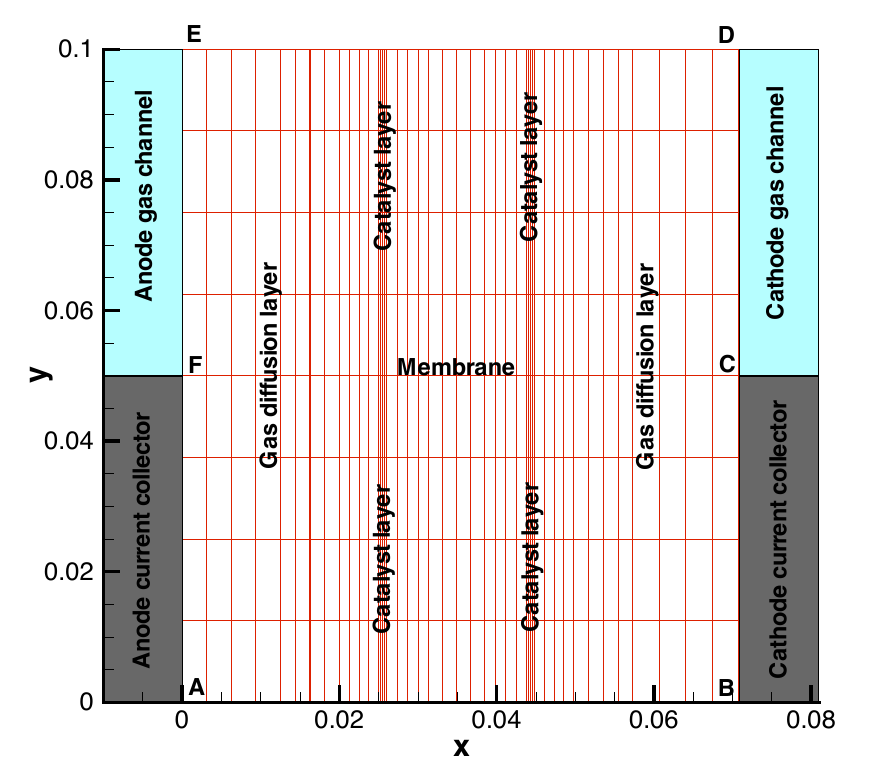
\includegraphics[width=10cm] {./figures/domain} 
\caption{Computational domain and initial grid used to solve the equations of the MEA model.}
\label{fig:domain_and_mesh}
\end{center}
\end{figure}

%---- Figures---
\begin{figure}[btp]
\begin{center}
%\includegraphics[width=6cm] {./figures/experimental_validation} 
\caption{Polarization curves from experimental data and numerical data at 75\% and 100\% RH.}
\label{fig:experimental_validation}
\end{center}
\end{figure}


\end{document}